\documentclass[a4paper]{article}

\usepackage[UTF8]{ctex}
\usepackage[a4paper,margin=1in]{geometry}
\usepackage{graphicx}
\usepackage{float}
\usepackage{listings}
\usepackage{booktabs}
\usepackage{color}
\usepackage{indentfirst}
\setlength{\parindent}{2em}
\usepackage{zhnumber}
\usepackage{adjustbox}
\usepackage{subcaption}
\usepackage{amsmath}
\usepackage{amssymb}
\usepackage{enumitem}
\usepackage{lmodern}
\usepackage{inconsolata}
\usepackage{multirow}
\usepackage{tikz}
\usetikzlibrary{positioning}
\usepackage{fancyhdr}
\usepackage{hyperref}
\usepackage{longtable} % 引入长表格宏包

% 配置lstlisting支持中文
\lstset{
    language=C,
    basicstyle=\footnotesize\ttfamily,
    breaklines=true,
    keywordstyle=\bfseries\color{blue},
    commentstyle=\itshape\color{green!50!black},
    stringstyle=\bfseries\color{red},
    numbers=left,
    numberstyle=\tiny\color{gray},
    frame=single,
    backgroundcolor=\color{gray!5},
    showstringspaces=false,
    keepspaces=true,
    tabsize=4,
    extendedchars=true,
    inputencoding=utf8,
    literate={，}{{\textcolor{green!50!black}{，}}}{1}
             {。}{{\textcolor{green!50!black}{。}}}{1}
             {：}{{\textcolor{green!50!black}{：}}}{1}
             {；}{{\textcolor{green!50!black}{；}}}{1}
             {（}{{\textcolor{green!50!black}{（}}}{1}
             {）}{{\textcolor{green!50!black}{）}}}{1}
             {【}{{\textcolor{green!50!black}{【}}}{1}
             {】}{{\textcolor{green!50!black}{】}}}{1}
}

\newcommand{\projname}{计算机网络实验}
\newcommand{\reporttitle}{计算机网络期末实验个人报告}
\newcommand{\groupno}{第一组}
\newcommand{\authorname}{马福泉}
\newcommand{\major}{计算机科学与技术}
\newcommand{\adviser}{谢逸}
\newcommand{\startdate}{2025年12月22日}
\newcommand{\labenddate}{2025年12月29日}
\newcommand{\labroom}{实验D402}

\pagestyle{fancy}
\fancyhf{}
\fancyhead[L]{\kaishu \projname}
\fancyhead[C]{\kaishu \reporttitle}
\fancyhead[R]{\kaishu \authorname}
\fancyfoot[C]{第 \thepage 页}
\renewcommand{\headrulewidth}{0.4pt}
\renewcommand{\footrulewidth}{0pt}


\begin{document}

% 封面
\begin{titlepage}
    \centering
    
\includegraphics[width=10cm]{img/SYSULogo.png} 
    \vspace{1em}
    \par
    {\Large \kaishu
        \par
        \projname
        \par
    }
    \vspace{3em}
    {\fontsize{40pt}{42pt}\kaishu \selectfont \boldmath \reporttitle\par}
    \vspace*{\fill}
    \begin{center}
    {\Large
    \makebox[5em][s]{姓名}:\underline{\makebox[15em][c]{\kaishu \authorname}}\\[1em]
    \makebox[5em][s]{学号}:\underline{\makebox[15em][c]{\kaishu 23336179}}\\[1em]
    \makebox[5em][s]{小组编号}:\underline{\makebox[15em][c]{\kaishu \groupno}}\\[1em]
    \makebox[5em][s]{专业}:\underline{\makebox[15em][c]{\kaishu \major}}\\[1em]
    \makebox[5em][s]{课程教师}:\underline{\makebox[15em][c]{\kaishu \adviser}}\\[1em]
    \makebox[5em][s]{起始日期}:\underline{\makebox[15em][c]{\kaishu \startdate}}\\[1em]
    \makebox[5em][s]{结束日期}:\underline{\makebox[15em][c]{\kaishu \labenddate}}\\[1em]
    \makebox[5em][s]{实验地点}:\underline{\makebox[15em][c]{\kaishu \labroom}}
    }
    \end{center}
    \vspace*{\fill}
\end{titlepage}

\section{承担的工作}
\subsection{主要负责工作}

\begin{enumerate}
    \item \textbf{交换机 VLAN 与 RSTP 配置及防环测试}：
    \begin{itemize}
        \item \textbf{二层网络基础构建}：负责交换机 S1 与 S2 的基础配置。在两台设备上分别创建了 VLAN 10 和 VLAN 20，根据拓扑需求，将连接 PC 的下行端口配置为 Access 模式，将交换机互联及上联路由器的端口配置为 Trunk 模式，并允许相应 VLAN 通过，确保了二层链路的逻辑隔离与连通。
        \item \textbf{RSTP 防环部署}：为了解决双链路互联可能引发的广播风暴，我在 S1 和 S2 上开启了 RSTP（快速生成树协议）。
        \item \textbf{环路测试验证}：在物理连接双网线后，通过 \texttt{display stp brief} 命令监控端口状态，成功观察到其中一条链路的端口转变为 \texttt{DISCARDING}（阻塞）状态，而另一条为 \texttt{FORWARDING}，从而证实了二层防环机制生效，避免了网络风暴。如下图 \ref{fig:rstp_test} 所示。
    \end{itemize}
    \begin{figure}[H]
        \centering
        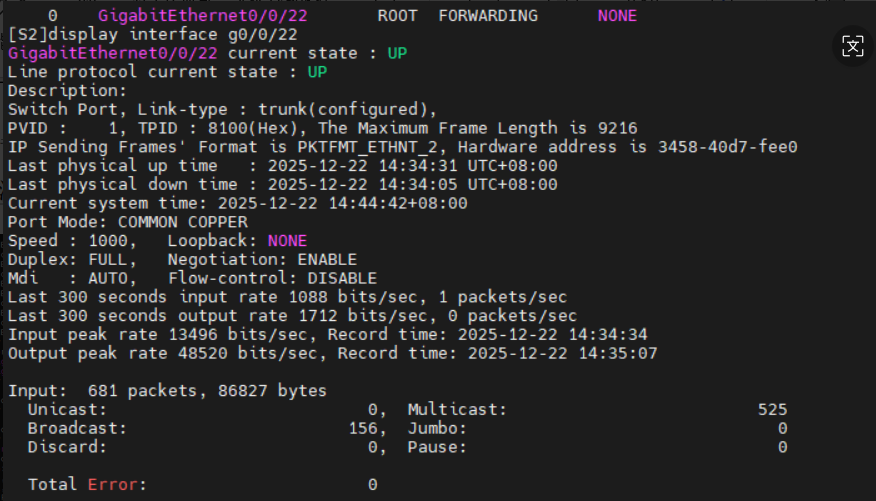
\includegraphics[width=0.7\textwidth]{img/0.png}
        \caption{RSTP 防环测试结果：端口状态显示一条链路被阻塞}
        \label{fig:rstp_test}
    \end{figure}


    \item \textbf{主机 H4 的部署与连通性保障}：
    \begin{itemize}
        \item 我全权负责实验中特殊节点 H4 (VLAN 20) 的配置与调试。由于题目要求 H4 在任何 ACL 策略下均不受限制，其网络配置的正确性至关重要。
        \item 如图 \ref{fig:h4_config} 所示，我将 H4 的 IP 地址配置为 192.168.20.4，网关指向 R1 的 VLAN 20 接口 (192.168.20.254)。
        \item 如图 \ref{fig:h4_success} 所示，在排除H4和队友的H5防火墙干扰后，成功验证了 H4 与远程主机 H5 (192.168.50.5) 的连通性，且平均延迟稳定在 1ms，证明接入层配置无误。
    \end{itemize}

    \begin{figure}[H]
        \centering
        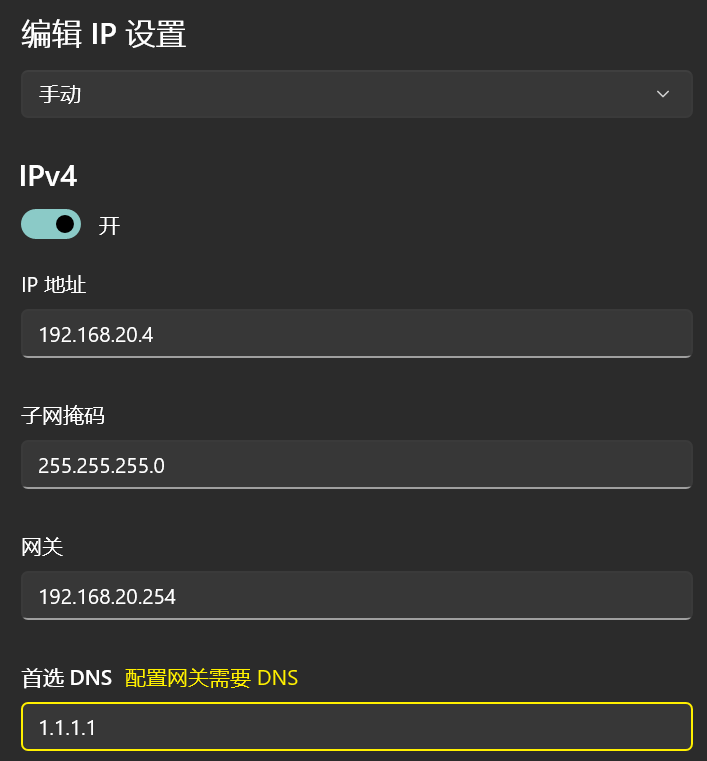
\includegraphics[width=0.7\textwidth]{img/1.png}
        \caption{H4 IP地址与网关配置}
        \label{fig:h4_config}
    \end{figure}

    \begin{figure}[H]
        \centering
        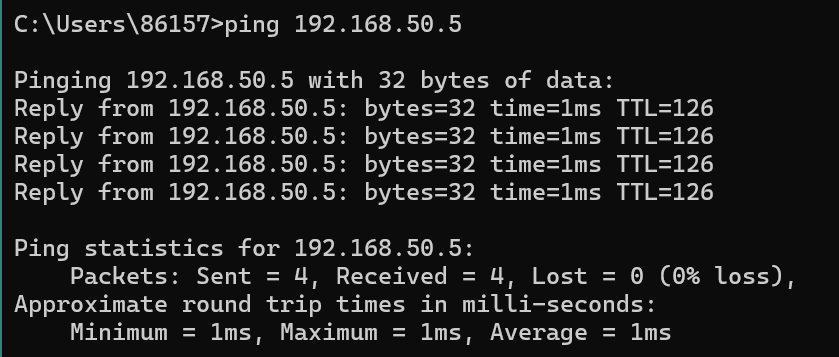
\includegraphics[width=0.7\textwidth]{img/2.png}
        \label{fig:h4_success}
        \caption{主机 H4 的配置与连通性测试结果}
    \end{figure}

\end{enumerate}

\subsection{次要的协助工作}

\begin{enumerate}
    \item \textbf{网络规划与 IP 地址设计}：
    \begin{itemize}
        \item 结合实验指导书的拓扑图进行详细分析，协助队友设计了如下全网 IP 地址分配表，合理划分了 VLAN 10（针对 H2）和 VLAN 20（针对 H1, H4），并规划了 R1 与 R2 之间的互联互通网段。
        \begin{table}[H]
            \centering
            \caption{实验网络 IP 地址与 VLAN 规划表}
            \label{tab:ip_plan}
            \resizebox{\textwidth}{!}{%
            \begin{tabular}{|c|c|c|c|c|c|}
            \hline
            \textbf{设备名称} & \textbf{接口} & \textbf{IP 地址} & \textbf{子网掩码} & \textbf{所属网段/VLAN} & \textbf{说明} \\ \hline
            \multirow{4}{*}{R1} & GE0/0/0 & 192.168.10.254 & 255.255.255.0 & VLAN 10 & VLAN 10 网关 \\ \cline{2-6} 
                                & GE0/0/1 & 192.168.20.254 & 255.255.255.0 & VLAN 20 & VLAN 20 网关 \\ \cline{2-6} 
                                & GE0/0/2 & 192.168.30.254 & 255.255.255.0 & 192.168.30.0/24 & 连接 H3 \\ \cline{2-6} 
                                & GE0/0/3 & 192.168.12.1 & 255.255.255.0 & 192.168.12.0/24 & R1-R2 互联 \\ \hline
            \multirow{2}{*}{R2} & GE0/0/0 & 192.168.12.2 & 255.255.255.0 & 192.168.12.0/24 & R1-R2 互联 \\ \cline{2-6} 
                                & GE0/0/1 & 192.168.50.254 & 255.255.255.0 & 192.168.50.0/24 & 连接 H5 \\ \hline
            H1 & Eth0 & 192.168.20.1 & 255.255.255.0 & VLAN 20 & H1 主机 \\ \hline
            H2 & Eth0 & 192.168.10.2 & 255.255.255.0 & VLAN 10 & H2 主机 \\ \hline
            H3 & Eth0 & 192.168.30.3 & 255.255.255.0 & 192.168.30.0/24 & H3 主机 \\ \hline
            H4 & Eth0 & 192.168.20.4 & 255.255.255.0 & VLAN 20 & H4 主机 \\ \hline
            H5 & Eth0 & 192.168.50.5 & 255.255.255.0 & 192.168.50.0/24 & H5 主机 \\ \hline
            \end{tabular}%
            }
        \end{table}
    \end{itemize}
    \item \textbf{Socket 通信程序测试}：
    \begin{itemize}
        \item \textbf{协议设计验证}：协助队友基于 Python 的 \texttt{socket} 库，测试调试了代码。针对 TCP 粘包问题，采用了“定长包头 (4字节长度) + 变长包体”的协议设计。在初期先调试了文本数据的封包与解包逻辑。如图 \ref{fig:socket_debug} 所示，这是程序初期调试成功的界面，可以看到包含了实验要求的中大文本。
        
        \begin{figure}[H]
            \centering
            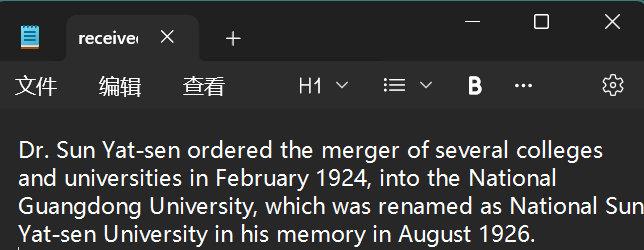
\includegraphics[width=0.8\textwidth]{img/4.png}
            \caption{Socket 通信程序开发初期调试：文本内容传输确认}
            \label{fig:socket_debug}
        \end{figure}
    \end{itemize}
\end{enumerate}

\section{遇到的困难及解决方法}

在实验过程中，我遇到了一些理论与实践结合上的挑战，特别是在ACL验证、路径分析以及防火墙设置方面，通过查阅资料和多次调试得以解决。

\begin{enumerate}
    \item \textbf{防火墙拦截导致的连通性假性故障}：
    \begin{itemize}
        \item \textbf{现象}：在确保路由表正确、ACL规则放行的情况下，H4 Ping H5 时依然出现了“请求超时”的错误，如图 \ref{fig:firewall_fail} 所示，导致我们一度怀疑 OSPF 配置错误。
        \item \textbf{原因分析}：经过 Wireshark 抓包分析，发现 ICMP 请求包已经到达目的主机，但没有回显应答。这通常是因为 Windows 操作系统的防火墙默认策略会拦截入站的 ICMP Echo Request 报文。
        \item \textbf{解决方案}：在目的主机 H5 上进入控制面板，暂时关闭 Windows 防火墙（或在高级安全设置中参加入站规则允许 ICMPv4）。修改设置后，再次 Ping 测试（如图 \ref{fig:h4_success} 所示），通信立即恢复。
    \end{itemize}

    \begin{figure}[H]
        \centering
        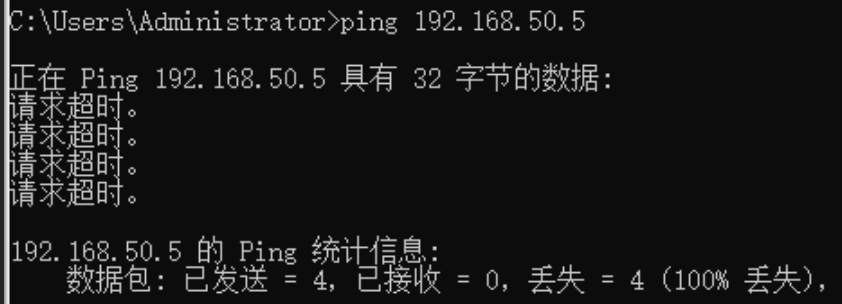
\includegraphics[width=0.7\textwidth]{img/3.png}
        \caption{防火墙拦截导致 Ping 请求超时（假性网络故障）}
        \label{fig:firewall_fail}
    \end{figure}

    \item \textbf{时间流控策略未生效的排查}：
    \begin{itemize}
        \item \textbf{现象}：在部署完基于时间的ACL后，我们试图验证“上午时段”H1访问H5的连通性，但Ping测试一直提示请求超时，策略似乎未按预期放行流量。
        \item \textbf{原因分析}：我们经过反复检查ACL语句逻辑并未发现错误。最终发现问题出在路由器的系统时钟上。由于模拟器中的路由器时间未与现实同步，导致当前系统时间不在定义的生效时间段内，数据包因此匹配失败并被默认规则丢弃。
        \item \textbf{解决方案}：我们通过 \texttt{clock datetime} 命令强制修改路由器系统时间至上午9点。修改后再次测试，H1与H5通信恢复正常。随后我们又模拟了下午和晚上的时间点，确认了策略能够随系统时间变化而正确切换。
    \end{itemize}

    \item \textbf{混淆了VLAN间通信的转发层级}：
    \begin{itemize}
        \item \textbf{现象}：H1 (VLAN 20) 和 H2 (VLAN 10) 均连接在同一台二层交换机上且能互通，这让我一度产生了它们是通过交换机直接进行二层转发的错觉。无法理解他们怎么能够跨VLAN通信。
        \item \textbf{原因分析}：VLAN的划分本质上就是为了隔离二层广播域。不同VLAN的主机即使物理距离很近，逻辑上也是隔离的，必须通过三层网关（路由器）进行路由转发才能通信。路径分析如下图 \ref{fig:vlan_path} 所示，H1发送数据包到H2时，数据包首先被发送到默认网关R1的VLAN 20接口，R1进行路由决策后，再从VLAN 10接口转发到H2，实现了跨VLAN通信。
        \begin{figure}[H]
            \centering
            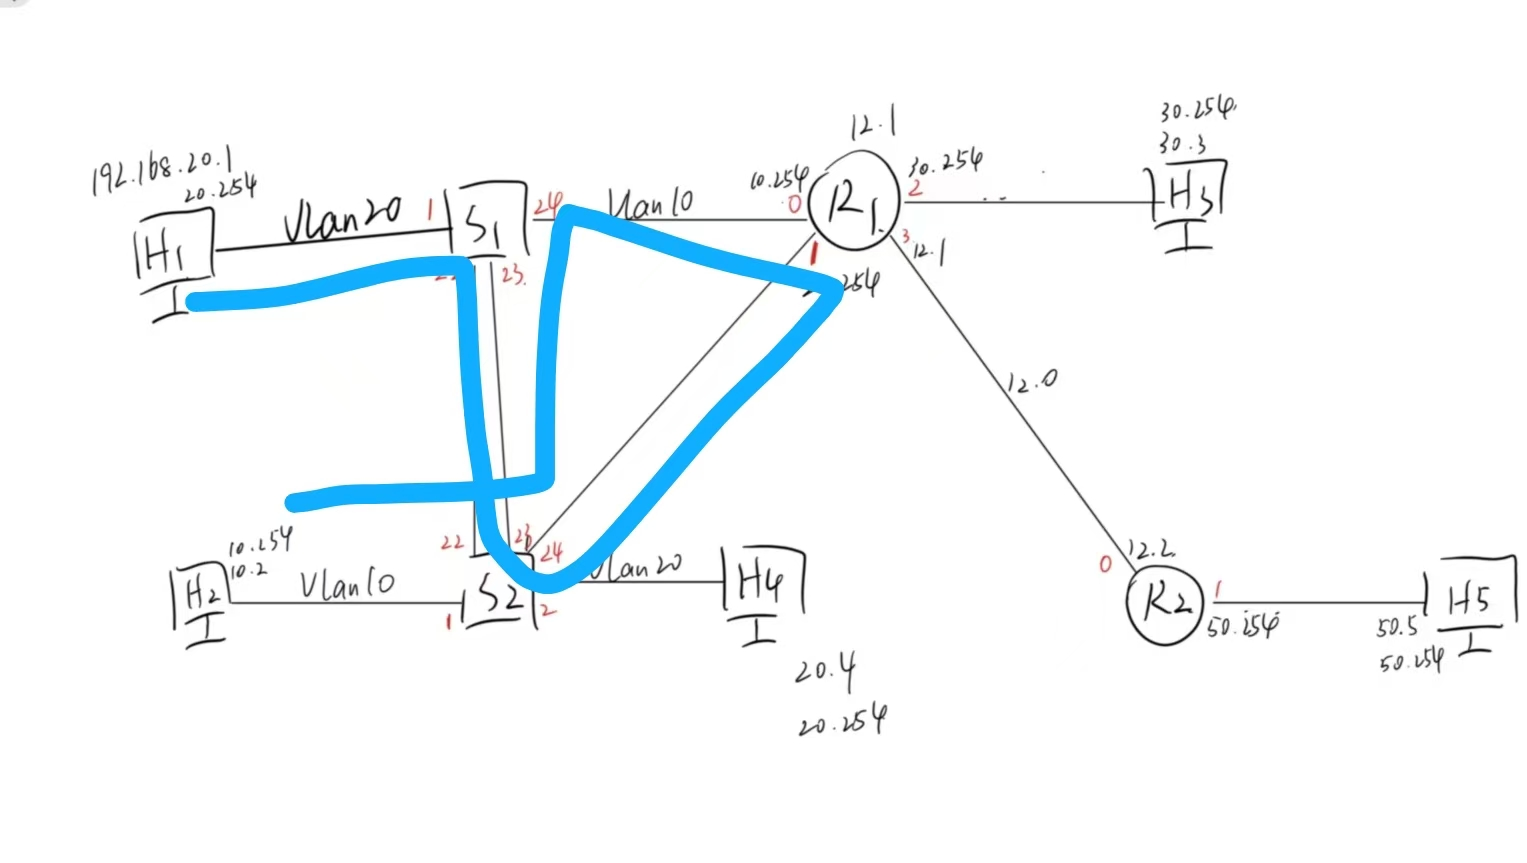
\includegraphics[width=0.7\textwidth]{img/6.png}
            \caption{VLAN间通信路径分析示意图}
            \label{fig:vlan_path}
        \end{figure}
        \item \textbf{解决方案}：经过队友的提醒，我理解了原理，为了验证该路径，我们在H1上运行了 \texttt{tracert} 命令追踪到达H2的路径。结果显示数据包的第一跳确实指向了网关R1 (192.168.20.254)，证实了流量是“绕道”路由器进行的转发，加深了我们对单臂路由原理的理解。如下图 \ref{fig:tracert} 所示。
        \begin{figure}[H]
        \centering
        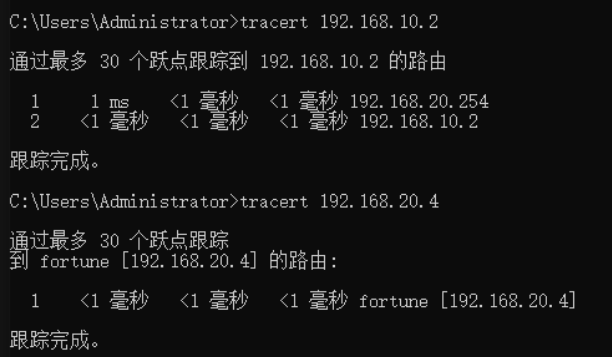
\includegraphics[width=0.7\textwidth]{img/5.png}
        \caption{H1 Tracert H2 路径分析结果：显示经过路由器 R1 实现跨VLAN通信}
        \label{fig:tracert}
    \end{figure}
    \end{itemize}
    
\end{enumerate}
\section{体会与总结}
\textbf{理论与实践的深度融合}：本次实验，我负责解决了二层环路风暴，目睹了生成树协议如何阻塞端口；亲自配置了OSPF邻居建立的过程，理解了链路状态数据库同步的意义。

\textbf{网络规划的重要性}：实验初期的IP地址规划表起到了决定性作用。清晰的网段划分（如VLAN 10/20与互联地址）减少了后续配置中的路由冲突和逻辑混乱。这让我明白优秀的网络工程始于周密的设计。

\textbf{跨层视角的建立}：通过Socket编程，我从应用层开发者的角度审视了底层网络。我意识到下层网络设备（路由器、交换机）为上层应用提供了透明、可靠的数据通路。这种跨越网络层到应用层的全局视野，对我未来的专业学习和工程实践具有重要的指导意义。
\end{document}